\documentclass[11pt,a4paper]{article}

\usepackage[T1]{fontenc}
\usepackage[utf8]{inputenc}
\usepackage[margin=2.4cm]{geometry}
\usepackage{graphicx}
\usepackage{booktabs}
\usepackage{amsmath}
\usepackage{amssymb}
\usepackage{xcolor}
\usepackage{float}
\usepackage[font=small,labelfont=bf]{caption}
\usepackage{enumitem}
\usepackage[hidelinks]{hyperref}

\graphicspath{{figures/}}

\definecolor{accent}{HTML}{1F4E79}
\definecolor{boxbg}{HTML}{F4F6F8}

\newcommand{\dE}{\ensuremath{\Delta E_{00}}}
\newcommand{\Cpk}{\ensuremath{C_{pk}}}
\newcommand{\um}{\ensuremath{\,\mu\mathrm{m}}}
\newcommand{\nm}{\ensuremath{\,\mathrm{nm}}}
\newcommand{\degC}{\ensuremath{^\circ\mathrm{C}}}

% A shaded box for plain-language asides.
\usepackage{mdframed}
\newmdenv[
  backgroundcolor=boxbg,
  linecolor=accent,
  linewidth=1pt,
  topline=false, bottomline=false, rightline=false,
  innerleftmargin=10pt, innertopmargin=8pt, innerbottommargin=8pt,
  skipabove=10pt, skipbelow=10pt
]{plainbox}

\title{\vspace{-1.2cm}\textbf{Predicting Colour Yield from Process Control Limits}\\[0.35em]
\large A physics-based capability study of anodizing and PVD thin-film finishing}
\author{Jnanadyuti Patra}
\date{18 September 2026}

\begin{document}
\maketitle

\begin{abstract}
\noindent
Manufactured products that must look identical --- a laptop lid, a watch case, a
phone frame --- get their colour from a surface finishing process, and that
process drifts. This study builds a physics model of two industrial finishing
routes, anodizing-and-dyeing and physical vapour deposition (PVD), and pushes
realistic process variation through them to predict what fraction of parts land
inside a colour specification. The two routes are found to fail in entirely
different places. A black anodized finish is almost immune to colour variation
($\Cpk = 16.7$) and is limited instead by film thickness ($\Cpk = 1.80$). A PVD
interference stack has no thickness problem at all, yet yields only
$56.4\,\%$ at realistic tolerances, with a single variable --- nitrogen
stoichiometry --- responsible for $69.8\,\%$ of the colour variance. Solving for
the control limits that would achieve $\Cpk \geq 1.33$ requires tightening
nitrogen control sixfold. A third result is that the colour a designer selects
is itself a capability decision: holding the anodizing process completely fixed
and changing only the dye moves yield from $100\,\%$ to $77.7\,\%$.
\end{abstract}

\vspace{-0.4cm}
\tableofcontents
\vspace{0.4cm}

% =====================================================================
\section{The problem, in plain language}

\subsection{Why this matters}

Pick up any anodized aluminium laptop or any coated stainless steel watch. It
has a colour. Now consider that the factory made a million of them, and every
single one has to be the \emph{same} colour --- close enough that a customer
holding two of them side by side cannot tell.

That is harder than it sounds, because colour is not painted on. It is the
by-product of a chemical or physical process running in a tank or a vacuum
chamber, and every one of those processes drifts. The acid bath warms up over a
shift. The dye gets consumed. A gas flow controller reads half a percent high.
None of these drifts is a fault; they are the normal breathing of a production
line. The question is whether the colour they produce still falls inside the
tolerance.

\begin{plainbox}
\textbf{The question this study answers.} Given how tightly a real production
line holds its process settings, what fraction of parts come out the right
colour --- and if the answer is not good enough, which single control should be
tightened first?
\end{plainbox}

This matters commercially because cosmetic rejects are expensive and late. A
part that fails a dimensional check fails at the machine. A part that fails a
\emph{cosmetic} check fails at the very end, after all the value has been added,
and it usually cannot be reworked.

\subsection{What gets built}

The study builds a computer model that runs the whole causal chain:

\begin{center}
\fbox{\parbox{0.92\textwidth}{\centering
process settings drift $\;\longrightarrow\;$ the film that grows changes
$\;\longrightarrow\;$ the light it reflects changes
$\;\longrightarrow\;$ the colour a human sees changes
$\;\longrightarrow\;$ some parts fall outside spec
}}
\end{center}

Because every link is physics rather than a curve fit, the model can be asked
questions no lookup table could answer --- for example, what happens at a
temperature nobody has tried yet.

\subsection{A glossary, for readers new to the field}

\begin{description}[leftmargin=0pt, style=nextline, itemsep=3pt]
  \item[Anodizing] An electrochemical process. An aluminium part is made the
  positive electrode in an acid bath, and a hard, porous oxide skin grows out of
  the metal's own surface. The pores can then be filled with dye, which is how
  anodized parts get colour. Used on most aluminium consumer electronics.

  \item[PVD (physical vapour deposition)] A vacuum process. A solid metal target
  is vaporised, and the vapour condenses on the part as an extremely thin film
  --- typically a few hundred nanometres, about a thousandth of a human hair.
  Reacting the vapour with nitrogen gas makes titanium nitride, a hard ceramic
  that happens to be gold-coloured. Used for watch cases, taps, and tooling.

  \item[Reflectance spectrum, $R(\lambda)$] The fraction of light a surface
  reflects, measured separately at each wavelength $\lambda$. This is the raw
  physical description of colour: an object looks red because its spectrum is
  high in the red and low elsewhere.

  \item[CIELAB] A colour coordinate system with three numbers: $L^*$ for
  lightness ($0$ black, $100$ white), $a^*$ for green-to-red, $b^*$ for
  blue-to-yellow. It is designed so that equal distances correspond roughly to
  equally visible differences.

  \item[\dE\ (CIEDE2000)] The standard measure of how different two colours look.
  Roughly, $\dE \approx 1$ is the smallest difference a trained observer can
  reliably see. Cosmetic specifications for consumer products are usually set at
  or below this value.

  \item[\Cpk\ (process capability index)] A single number saying how comfortably
  a process fits inside its tolerance. $\Cpk = 1.0$ means the tolerance band is
  exactly as wide as the process spread; $\Cpk = 1.33$ is the usual consumer
  electronics gate and corresponds to roughly $32$ defective parts per million.
  Below $1.0$ the process is not fit for the specification.

  \item[DOE (design of experiments)] A structured plan for varying several
  settings at once, so that their individual and combined effects can be
  separated from a small number of runs rather than a huge number.
\end{description}

% =====================================================================
\section{Method}

\subsection{The shared pipeline}

Both finishing routes are modelled independently up to the point where they
produce a reflectance spectrum, after which they share one common path to
colour and capability:

\begin{equation*}
\underbrace{\text{process variation}}_{\text{Monte Carlo}}
\;\longrightarrow\;
\underbrace{\text{physics}}_{\substack{\text{anodizing kinetics}\\ \text{or transfer matrix}}}
\;\longrightarrow\;
R(\lambda)
\;\longrightarrow\;
\underbrace{L^*a^*b^*}_{\text{CIE}}
\;\longrightarrow\;
\dE
\;\longrightarrow\;
\Cpk
\;\longrightarrow\;
\text{yield}
\end{equation*}

Sharing the colour engine is what makes the two routes directly comparable: any
difference in the final capability number is attributable to the physics of the
finish, not to differences in how colour was computed.

\subsection{From a spectrum to a colour}

Human colour vision has three receptor types. The CIE formalises this with three
\emph{colour matching functions} $\bar{x}(\lambda)$, $\bar{y}(\lambda)$,
$\bar{z}(\lambda)$, which describe the sensitivity of a standard observer.
Multiplying the reflectance by the illuminating light $S(\lambda)$ and by each
of these, then integrating, yields the tristimulus values:

\begin{equation}
X = k\!\int R(\lambda)\,S(\lambda)\,\bar{x}(\lambda)\,\mathrm{d}\lambda,
\qquad
k = \frac{100}{\int S(\lambda)\,\bar{y}(\lambda)\,\mathrm{d}\lambda}
\end{equation}

with $Y$ and $Z$ defined analogously. The illuminant used throughout is D65,
standard average daylight. $XYZ$ is then converted to CIELAB through a cube-root
compression that mimics the eye's non-linear lightness response, and two colours
are compared using the CIEDE2000 formula,

\begin{equation}
\dE = \sqrt{
\left(\frac{\Delta L'}{k_L S_L}\right)^{\!2}
+\left(\frac{\Delta C'}{k_C S_C}\right)^{\!2}
+\left(\frac{\Delta H'}{k_H S_H}\right)^{\!2}
+ R_T \frac{\Delta C'}{k_C S_C}\frac{\Delta H'}{k_H S_H}}
\end{equation}

whose weighting terms $S_L, S_C, S_H$ and rotation term $R_T$ correct for the
fact that the eye's sensitivity depends on where in colour space the comparison
is being made --- it is far more sensitive to a shift in a pale grey than to the
same numerical shift in a saturated blue.

\subsection{Route 1: anodizing}

Anodic oxide grows by Faraday's law from the anodizing current, while the acid
simultaneously dissolves it back. The net growth is the difference:

\begin{equation}
\frac{\mathrm{d}x}{\mathrm{d}t}
= \underbrace{\frac{M_\mathrm{ox}\, j\, \eta}{z F \rho_\mathrm{ox}}}_{\text{electrochemical growth}}
\;-\;
\underbrace{k_0 \exp\!\left(-\frac{E_a}{RT}\right)[\mathrm{H_2SO_4}]^m}_{\text{chemical back-dissolution}}
\label{eq:anodize}
\end{equation}

with $M_\mathrm{ox} = 101.96$ g/mol for $\mathrm{Al_2O_3}$, $z = 6$ (forming one
$\mathrm{Al_2O_3}$ unit transfers six electrons), and
$\rho_\mathrm{ox} \approx 3.1$ g/cm$^3$ --- below dense sapphire, because the
anodic film is porous and partly hydrated.

\begin{plainbox}
\textbf{Why bath temperature dominates.} The second term in
Eq.~\eqref{eq:anodize} is Arrhenius, so it roughly doubles for every
$+10\degC$. A bath that drifts warm therefore does two bad things at once: it
thins the film, and it widens the pores. The part comes out lighter and duller.
No other single variable has this double effect, which is why temperature
control is the first thing any anodizing line invests in.
\end{plainbox}

The dye lives in the pores, so dye loading scales with pore volume, that is,
with porosity multiplied by thickness. Uptake saturates exponentially with
immersion time and peaks near pH 5.5, where acid dyes are most readily adsorbed
by the amphoteric oxide.

A dyed anodic film is a \emph{bulk absorber}, not an interference filter. Light
crosses the film, reflects off the aluminium underneath, and crosses back, so
the Beer--Lambert law applies over a double pass:

\begin{equation}
R(\lambda) = R_\mathrm{surf}
+ \left(1 - R_\mathrm{surf}\right)^2 R_\mathrm{Al}(\lambda)\,
  e^{-2\varepsilon(\lambda)\,c\,x}
\end{equation}

Because there is no interference term, dyed anodizing barely changes colour with
viewing angle --- the exact opposite of the PVD stack considered next.

\begin{figure}[H]
\centering
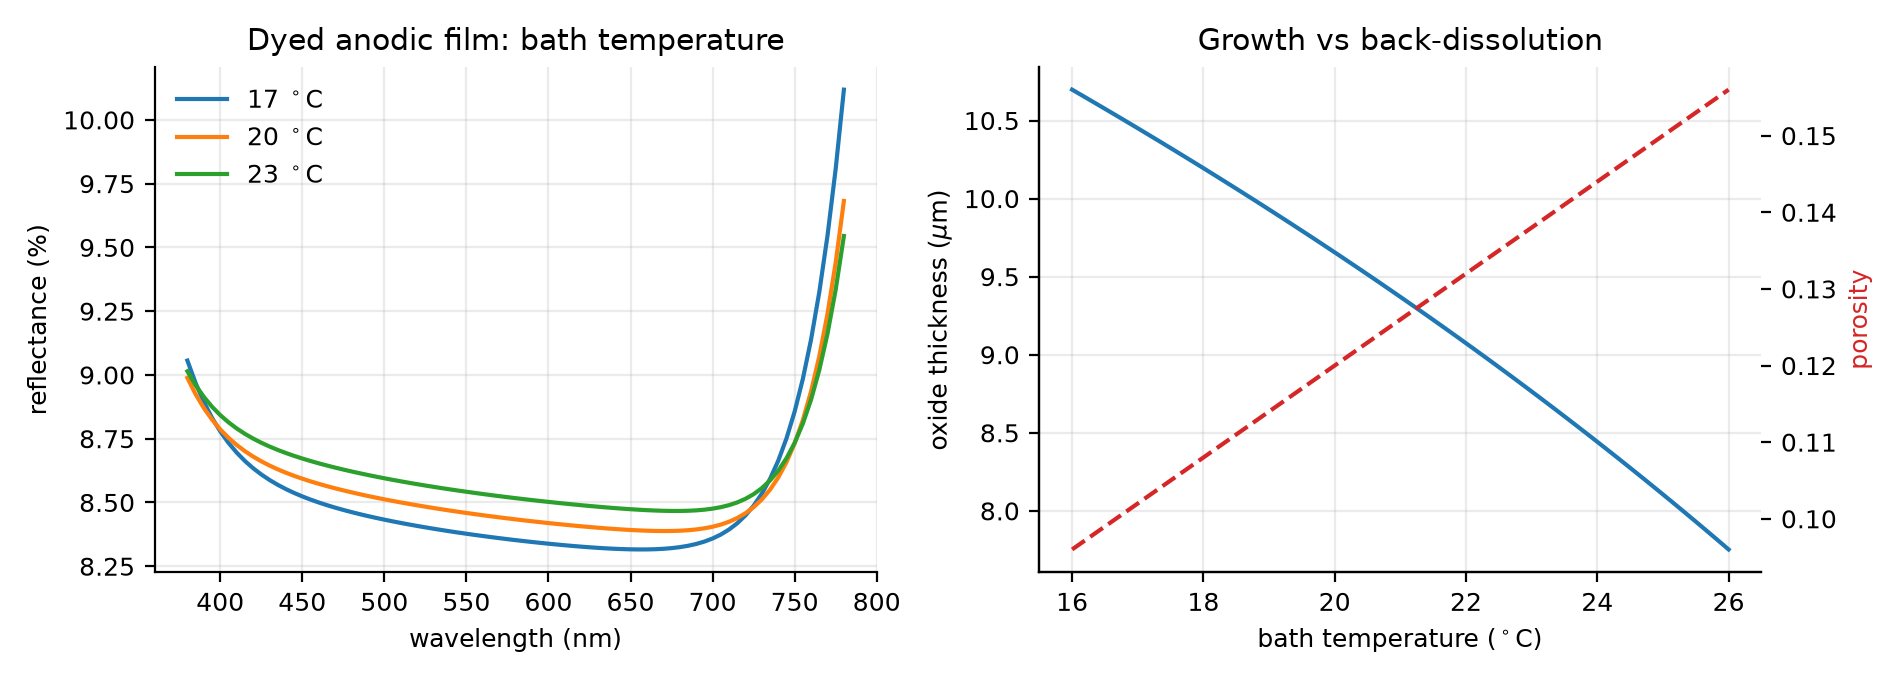
\includegraphics[width=\textwidth]{anodize_physics.png}
\caption{Left: the reflectance of a black-dyed film across a $\pm 3\degC$ bath
excursion. Right: the competition in Eq.~\eqref{eq:anodize} --- as the bath
warms, back-dissolution accelerates and thickness falls (blue), while porosity
rises (red, dashed).}
\end{figure}

\subsection{Route 2: PVD thin films}

A PVD coating is a stack of layers each a few hundred nanometres thick, which is
comparable to the wavelength of visible light. Light reflected from the top of a
layer therefore interferes with light reflected from its bottom, and the colour
depends on the whole stack rather than on any one surface.

The standard treatment assigns each layer a characteristic matrix,

\begin{equation}
M_j =
\begin{bmatrix}
\cos\delta_j & \dfrac{i\sin\delta_j}{\eta_j}\\[1.1em]
i\,\eta_j \sin\delta_j & \cos\delta_j
\end{bmatrix},
\qquad
\delta_j = \frac{2\pi\, t_j\, N_j \cos\theta_j}{\lambda}
\end{equation}

where $N_j = n_j - ik_j$ is the complex refractive index and $\eta_j$ the tilted
optical admittance. Multiplying the matrices maps the substrate admittance to
the front surface, giving

\begin{equation}
\begin{bmatrix} B\\ C\end{bmatrix}
= \left(\prod_j M_j\right)\begin{bmatrix} 1\\ \eta_\mathrm{sub}\end{bmatrix},
\qquad
Y = \frac{C}{B},
\qquad
R = \left|\frac{\eta_0 - Y}{\eta_0 + Y}\right|^2
\end{equation}

This is the same calculation performed by the commercial thin-film design
packages Essential Macleod and TFCALC.

\begin{plainbox}
\textbf{A sign convention that silently destroys the answer.} Tabulated optical
constants are published as $N = n + ik$. The matrix formulation above expects
$N = n - ik$. Feeding the first into the second turns every absorbing layer into
a \emph{gain} medium: the code runs, the plots look plausible, and reflectance
quietly exceeds $100\,\%$. This was caught here by a test asserting
$0 \leq R \leq 1$ for every stack at every angle, and that test is retained
precisely because the failure is invisible without it.
\end{plainbox}

The colour of a bulk nitride is controlled by its \emph{composition}, not its
thickness. Titanium nitride absorbs strongly enough that past roughly
$150\nm$ the film is optically opaque and the substrate beneath it becomes
irrelevant. The variable that actually matters is the stoichiometry $x$ in
$\mathrm{TiN}_x$, set on the tool by nitrogen partial pressure. As $x$ falls
below one the film is nitrogen-starved and metal-rich: more free carriers raise
the plasma frequency, the reflectance edge moves blue, and the gold drifts
toward metallic silver.

\begin{figure}[H]
\centering
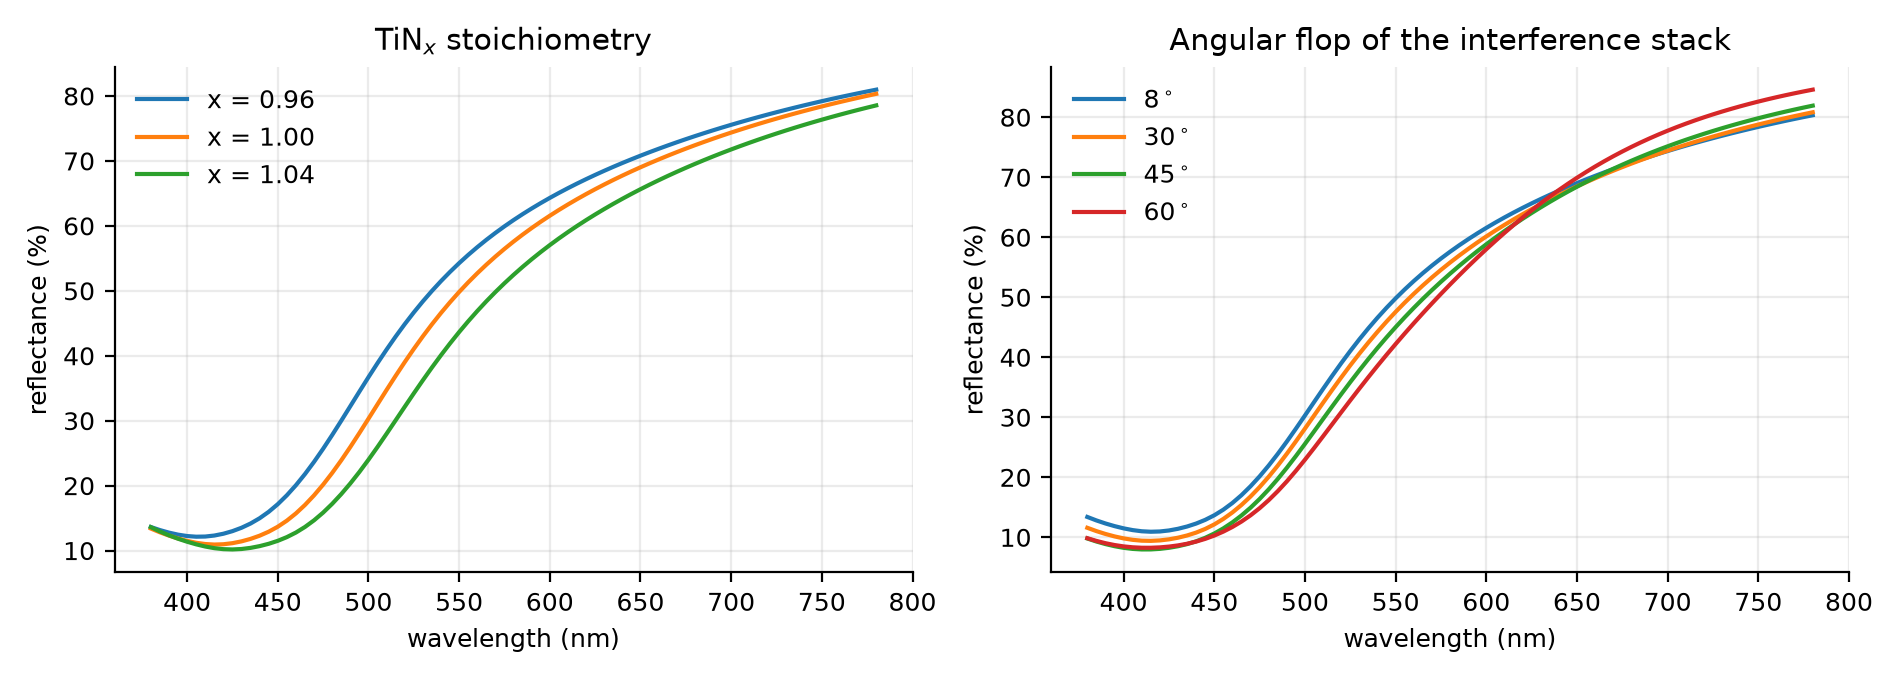
\includegraphics[width=\textwidth]{pvd_physics.png}
\caption{Left: reflectance of the PVD stack across a $\pm 4\,\%$ swing in
nitrogen stoichiometry. Right: angular colour shift (``flop'') of the same
interference stack --- the reason a part can pass inspection face-on and fail at
a chamfer.}
\end{figure}

\subsection{Propagating variation}

Each process input is assigned a control tolerance, interpreted as a
$\pm 3\sigma$ band, and sampled from a normal distribution. Every sample is
pushed through the forward model. Capability follows as

\begin{equation}
\Cpk = \frac{\min\left(\mathrm{USL} - \mu,\; \mu - \mathrm{LSL}\right)}{3\sigma},
\qquad
\Cpk^\mathrm{upper} = \frac{\mathrm{USL} - \mu}{3\sigma}
\end{equation}

the second form applying to \dE, for which there is no such thing as too little
colour error. Inputs are ranked by standardised regression coefficients, which
give the response change per standard deviation of input and therefore already
fold in both the physical sensitivity and the current control spread. That is
the correct ranking for deciding which tolerance to buy down.

\subsection{Experimental design}

A Box--Behnken design is used throughout. Unlike a central composite design it
places no run outside the stated factor range, which matters for a real bath:
axial points would demand acid concentrations the line cannot hold. A full
quadratic response surface is fitted on coded levels, so that coefficient
magnitudes are directly comparable.

% =====================================================================
\section{Verification}

Before any result is reported, the implementation is checked against published
values. The suite contains 62 tests; the load-bearing ones are:

\begin{table}[H]
\centering
\small
\begin{tabular}{@{}p{0.44\textwidth}p{0.50\textwidth}@{}}
\toprule
\textbf{Check} & \textbf{Result} \\
\midrule
All 13 CIEDE2000 reference pairs of Sharma, Wu \& Dalal (2005) & Reproduced to
within $10^{-4}$. These pairs exist specifically to exercise the hue-wraparound
and rotation terms that naive implementations get wrong. \\
\addlinespace
Perfect reflecting diffuser under D65 & Returns exactly $L^*=100$,
$a^*=b^*=0$. \\
\addlinespace
D65 white point & $(95.047,\,100,\,108.883)$, matching the CIE tabulation. \\
\addlinespace
$0 \leq R \leq 1$ for every stack at every angle & Passes; this is the check
that caught the sign-convention error. \\
\addlinespace
Nominal Type II recipe ($1.5$ A/dm$^2$, $30$ min, $20\degC$, $180$ g/L) &
Returns $9.66\um$ against the $\sim\!10\um$ industry specification. This is the
calibration anchor for the entire anodizing model. \\
\addlinespace
Back-dissolution temperature dependence & Verified to fall between $1.8\times$
and $3.0\times$ per $+10\degC$. \\
\addlinespace
Response-surface fitter on a known quadratic & Recovers every coefficient
exactly, $R^2 = 1$. \\
\bottomrule
\end{tabular}
\caption{Verification summary. All checks are automated and run in continuous
integration.}
\end{table}

% =====================================================================
\section{Results}

\subsection{Anodizing: colour is easy, thickness is not}

At the nominal window with a black dye, the process is comfortably capable on
colour and marginal on thickness.

\begin{table}[H]
\centering
\begin{tabular}{@{}lrrrr@{}}
\toprule
\textbf{Response} & \textbf{Mean} & \textbf{$\sigma$} & \textbf{Spec} & \textbf{\Cpk} \\
\midrule
\dE\ vs colour master & $0.032$ & $0.019$ & $\leq 1.0$ & $17.04$ \\
Oxide thickness       & $9.653\um$ & $0.307\um$ & $8$--$12\um$ & $1.80$ \\
\midrule
\multicolumn{4}{@{}l}{Combined yield} & $100.00\,\%$ \\
\bottomrule
\end{tabular}
\caption{Anodizing capability, $n=6000$ Monte Carlo samples.}
\end{table}

The Box--Behnken response surface fits thickness essentially perfectly
($R^2 = 0.99999$) and colour well ($R^2 = 0.932$). The thickness model is
dominated by linear terms in current density, bath temperature and acid
concentration, exactly as Eq.~\eqref{eq:anodize} demands.

\begin{figure}[H]
\centering
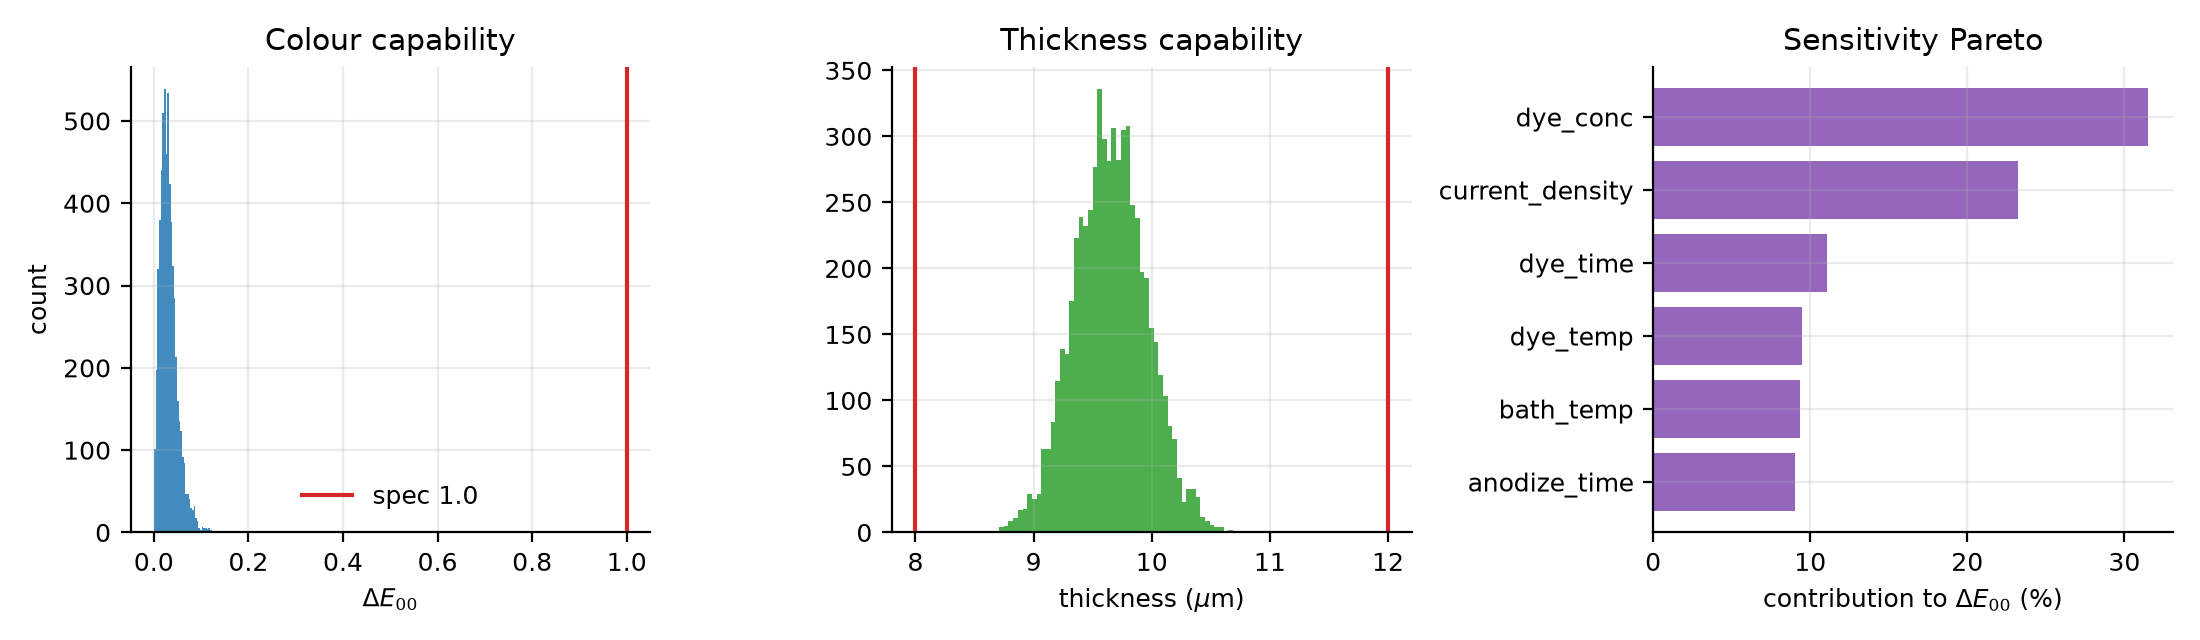
\includegraphics[width=\textwidth]{anodize_capability.png}
\caption{Anodizing capability. Colour (left) sits far inside its limit;
thickness (centre) consumes most of its window; the Pareto (right) identifies
dye concentration and current density as the leading contributors to colour
variation.}
\end{figure}

\subsection{The colour itself is a capability decision}

The most consequential result in this study comes from changing nothing about
the process. Holding the window, the tolerances and the sample size fixed, and
varying only which dye is in the tank:

\begin{table}[H]
\centering
\begin{tabular}{@{}lrrrr@{}}
\toprule
\textbf{Dye} & \textbf{Mean \dE} & \textbf{$\sigma$} & \textbf{\Cpk} & \textbf{Yield} \\
\midrule
Black          & $0.032$ & $0.019$ & $16.68$ & $100.00\,\%$ \\
Graphite grey  & $0.203$ & $0.158$ & $1.68$  & $99.96\,\%$ \\
Gold / bronze  & $0.549$ & $0.415$ & $0.36$  & $85.20\,\%$ \\
Red            & $0.566$ & $0.427$ & $0.34$  & $84.24\,\%$ \\
Blue           & $0.668$ & $0.512$ & $0.22$  & $77.72\,\%$ \\
\bottomrule
\end{tabular}
\caption{Identical process, identical tolerances, different dye.}
\end{table}

A saturated black sits deep in Beer--Lambert saturation: the exponential has
already bottomed out, so bath noise moves the reflectance hardly at all. Pale
and chromatic finishes sit on the steep part of the same exponential, where the
same noise produces a visible shift.

\begin{plainbox}
\textbf{Implication.} Yield swings by 22 percentage points with no process
change whatsoever. The decision that caused it was made in a design review, by
someone choosing a colour, long before any process engineer saw the part. This
argues for capability analysis being run \emph{at colour selection}, not after
the line is commissioned.
\end{plainbox}

\begin{figure}[H]
\centering
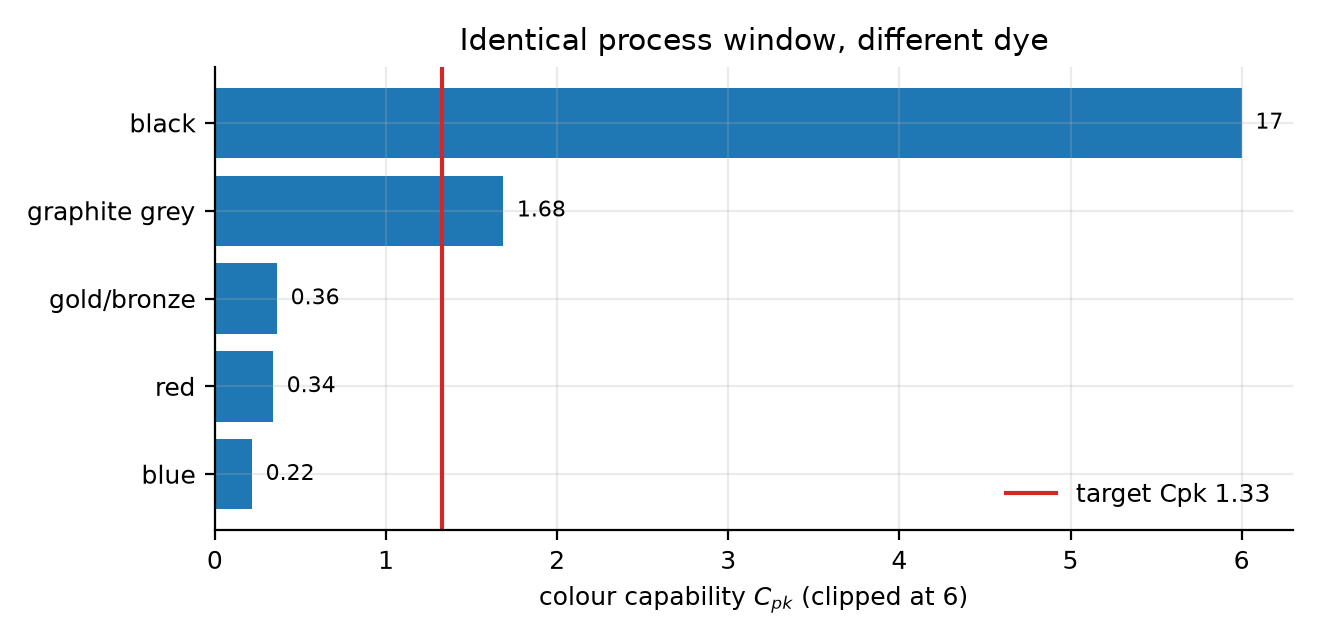
\includegraphics[width=0.72\textwidth]{anodize_dye_robustness.png}
\caption{Colour capability by dye choice under an identical process window. Only
black and graphite clear the $\Cpk = 1.33$ gate.}
\end{figure}

\begin{figure}[H]
\centering
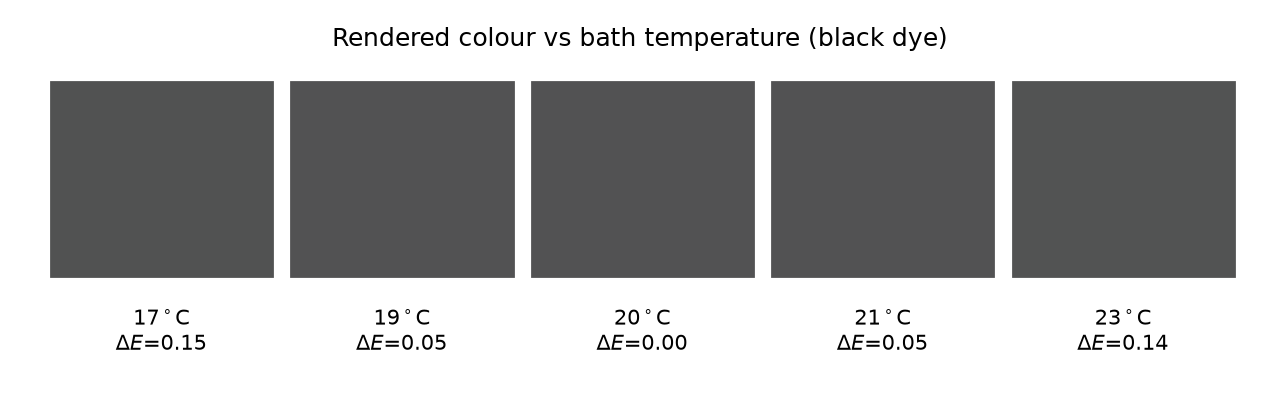
\includegraphics[width=\textwidth]{anodize_swatches.png}
\caption{Rendered appearance across a $\pm 3\degC$ bath excursion, with the
corresponding \dE. Swatches are computed from the simulated spectra through the
same CIE pipeline, then converted to sRGB for display.}
\end{figure}

\subsection{PVD: one variable dominates, and it is not thickness}

The PVD interference stack fails at tolerances that would be entirely normal on
a production tool.

\begin{table}[H]
\centering
\begin{tabular}{@{}lrrr@{}}
\toprule
\textbf{Quantity} & \textbf{Value} & \multicolumn{2}{l}{\textbf{Variance share}} \\
\midrule
Mean \dE                 & $1.042$   & Stoichiometry   & $69.8\,\%$ \\
$\sigma_{\dE}$           & $0.773$   & Overcoat thickness & $27.8\,\%$ \\
Colour \Cpk              & $-0.018$  & TiN thickness   & $2.5\,\%$ \\
Yield against $\dE \leq 1.0$ & $56.4\,\%$ & & \\
\bottomrule
\end{tabular}
\caption{PVD capability for the stack air / SiO$_2$ $90\nm$ / TiN $300\nm$ /
Ti $80\nm$ / SS304, $n=6000$.}
\end{table}

A negative \Cpk\ means the process mean already sits outside the specification
limit --- the average part is a reject. The response surface for \dE\ fits well
($R^2 = 0.996$, adjusted $0.989$) and is dominated by \emph{quadratic} terms in
stoichiometry, meaning the colour penalty grows faster than linearly as
nitrogen control drifts in either direction.

Greedily tightening the dominant tolerance until $\Cpk \geq 1.33$ converges in
18 rounds:

\begin{table}[H]
\centering
\begin{tabular}{@{}lrrl@{}}
\toprule
\textbf{Control} & \textbf{Current} & \textbf{Required} & \textbf{Change} \\
\midrule
TiN stoichiometry (nitrogen flow) & $\pm 0.040$  & $\pm 0.0067$ & $6.0\times$ tighter \\
SiO$_2$ overcoat thickness        & $\pm 8.0\nm$ & $\pm 3.0\nm$ & $2.7\times$ tighter \\
TiN thickness                     & $\pm 20\nm$  & $\pm 20\nm$  & unchanged \\
\bottomrule
\end{tabular}
\caption{Control limits required to reach $\Cpk = 1.33$.}
\end{table}

\begin{plainbox}
\textbf{The counter-intuitive part.} TiN thickness is the variable an engineer
would instinctively control, and it is almost irrelevant --- it accounts for
$2.5\,\%$ of the colour variance and its tolerance never needs tightening. The
film is optically opaque past roughly $150\nm$, so adding more of it changes
nothing an observer can see. Composition is the real lever, and composition is
controlled by a gas flow, not by a deposition timer.
\end{plainbox}

\begin{figure}[H]
\centering
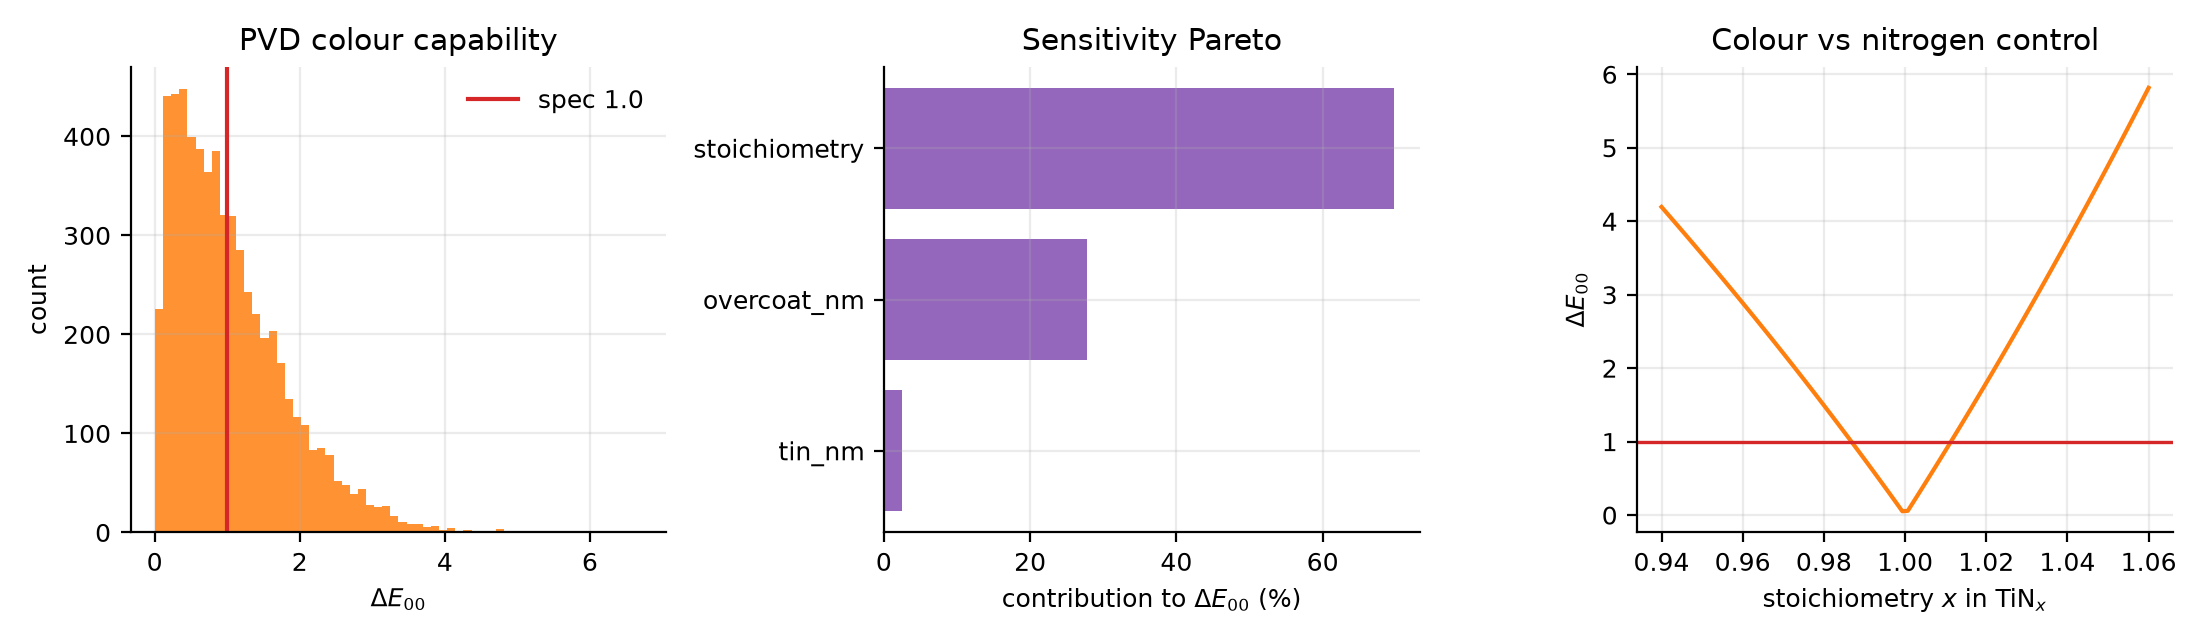
\includegraphics[width=\textwidth]{pvd_capability.png}
\caption{PVD capability. A large fraction of the simulated distribution (left)
lies beyond the specification. Stoichiometry dominates the Pareto (centre). The
colour penalty versus nitrogen control (right) is steeply quadratic, so
symmetric drift in either direction is punished.}
\end{figure}

\begin{figure}[H]
\centering
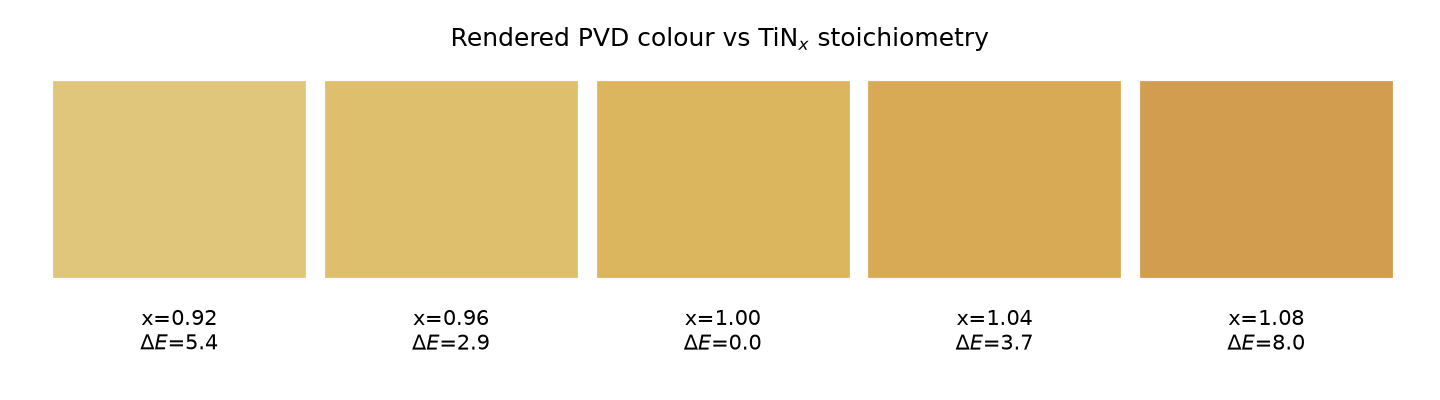
\includegraphics[width=\textwidth]{pvd_swatches.png}
\caption{Rendered PVD appearance across the stoichiometry range. A $\pm 8\,\%$
composition swing takes the finish from pale champagne to warm bronze.}
\end{figure}

\subsection{The two routes fail differently}

\begin{table}[H]
\centering
\begin{tabular}{@{}lll@{}}
\toprule
 & \textbf{Anodize + black dye} & \textbf{PVD interference stack} \\
\midrule
Binding constraint   & Film thickness      & Composition \\
Colour \Cpk          & $16.68$             & $-0.018$ \\
Limiting \Cpk        & $1.80$ (thickness)  & $-0.018$ (colour) \\
Dominant variable    & Current density, dye conc. & Nitrogen stoichiometry \\
Angular colour shift & Negligible (bulk absorber) & Significant (interference) \\
What to instrument   & Bath temperature, coating thickness gauge & Mass-flow control, optical monitor \\
\bottomrule
\end{tabular}
\caption{Comparative failure modes.}
\end{table}

A control plan written for one route is close to useless for the other. The
anodizing line needs thickness metrology and temperature control; the PVD line
needs gas-flow precision and in-chamber optical monitoring. Neither conclusion
is reachable without modelling the physics --- both routes produce ``a coloured
part'', and their process sheets look superficially similar.

% =====================================================================
\section{Limitations}

These results are simulation. Stating the boundaries precisely is part of the
result.

\begin{enumerate}[leftmargin=1.4em, itemsep=4pt]
  \item \textbf{Optical constants are representative literature fits}, not
  measurements of a specific supplier's coating. They reproduce the correct
  colour family and the correct dispersion shape, which is what a
  \emph{sensitivity} study requires: the conclusions concern how strongly colour
  responds to process variation, and that is governed by stack geometry and the
  shape of $n(\lambda)$ rather than by the third decimal place of any oscillator
  parameter. Absolute colour prediction against a physical master would require
  measured $n,k$ data, which the code accepts as a drop-in replacement.

  \item \textbf{The dye-uptake and porosity relations are phenomenological.}
  They are fitted to published Type II behaviour, not derived from first
  principles. Trends are trustworthy; absolute dye loadings are not.

  \item \textbf{Capability here is short-term.} Samples are drawn at fixed
  nominal settings, so what is computed is within-batch capability. Real
  long-term $P_{pk}$ on a line will be worse, because it additionally carries
  drift between bath changes, rack position, and operator.

  \item \textbf{No experimental validation.} No coupons were anodized and no
  spectrophotometer readings were taken. This is the single largest gap, and the
  natural next step. The code is deliberately structured so that a measured
  dataset drops directly into the existing comparison path.
\end{enumerate}

% =====================================================================
\section{Conclusions}

\begin{enumerate}[leftmargin=1.4em, itemsep=4pt]
  \item A single physics-to-colour-to-capability pipeline can serve two
  physically unrelated finishing routes, making them directly comparable on the
  only metric that matters commercially --- yield against a colour
  specification.

  \item The PVD interference stack studied here is not capable at realistic
  tolerances ($56.4\,\%$ yield, $\Cpk = -0.018$). Reaching $\Cpk = 1.33$ requires
  sixfold tighter nitrogen control, and no improvement whatsoever in the
  thickness control an engineer would instinctively tighten first.

  \item Anodized black is colour-robust and thickness-limited; the constraint
  and therefore the entire control strategy is the opposite of the PVD case.

  \item Cosmetic capability should be assessed at the point of \emph{colour
  selection}. Changing only the dye, with the process held completely fixed,
  moved yield from $100\,\%$ to $77.7\,\%$. That is a larger effect than most
  process improvements could recover, and it is free to avoid if it is
  considered early enough.
\end{enumerate}

% =====================================================================
\section*{Reproducibility}
\addcontentsline{toc}{section}{Reproducibility}

Every number and figure in this report is regenerated by a single command:

\begin{center}
\texttt{python scripts/run\_study.py}
\end{center}

The test suite (\texttt{python -m pytest}, 62 tests) runs in continuous
integration on Python 3.10--3.12, and the study itself is re-executed on every
push, so the document and the code cannot drift apart. The design tables are
also exported as JMP-ready CSV together with a JSL script that reconstructs the
response-surface analysis, prediction profiler and contour profiler directly.

% =====================================================================
\begin{thebibliography}{9}
\small

\bibitem{sheasby} Sheasby, P.~G. and Pinner, R.
\emph{The Surface Treatment and Finishing of Aluminium and its Alloys},
6th ed., ASM International / Finishing Publications, 2001.

\bibitem{macleod} Macleod, H.~A.
\emph{Thin-Film Optical Filters}, 4th ed., CRC Press, 2010.

\bibitem{sharma} Sharma, G., Wu, W. and Dalal, E.~N.
``The CIEDE2000 colour-difference formula: implementation notes, supplementary
test data, and mathematical observations.''
\emph{Color Research \& Application} \textbf{30}(1), 21--30, 2005.

\bibitem{wyman} Wyman, C., Sloan, P.-P. and Shirley, P.
``Simple analytic approximations to the CIE XYZ colour matching functions.''
\emph{Journal of Computer Graphics Techniques} \textbf{2}(2), 1--11, 2013.

\bibitem{montgomery} Montgomery, D.~C.
\emph{Design and Analysis of Experiments}, 10th ed., Wiley, 2019.

\bibitem{patsalas} Patsalas, P. and Logothetidis, S.
``Optical, electronic and transport properties of nanocrystalline titanium
nitride thin films.''
\emph{Journal of Applied Physics} \textbf{90}, 4725, 2001.

\bibitem{cie} CIE.
\emph{Colorimetry}, 4th ed., CIE 015:2018, Commission Internationale de
l'\'Eclairage, 2018.

\end{thebibliography}

\end{document}
